% Lezione 3.1
\documentclass[../template]{subfiles}

\begin{document}
\section{Architetture Avanzate}
\subsection{Prestazione dei calcolatori}
Con benchmark si intende un set di programmi differenti tra loro, che rappresentano
a grandi linee task frequenti eseguiti dal calcolatore.
Per comparare le prestazioni di diversi calcolatori, vengono paragonati
i tempi di esecuzione del benchmark.

\def\tcpu{T_\text{cpu}}

\subsection{Prestazione della CPU}
Considerato l'intero tempo di esecuzione di um programma, viene definito tempo di CPU, il tempo in cui effettivamente
quest'ultima è impiegata nel task: $\tcpu = N_{cc} T_{ck}$, dove $N_{cc}$ è il numero di cicli di clock.
\\
Il modello più semplice per calcolarlo è il CPI (\textit{Clock Per Instruction}): quanti cicli di clock servono in media
per un'istruzione: $\mathit{CPI} = N_{cc}/N$ dove $N$ è il numero di istruzioni in un programma.

Per calcolare il CPI medio, occorre conoscere il CPI di ogni istruzione, e la frequenza con la quale l'istruzione
$i$-esima viene eseguita $F_i$.
\[
    \mathit{CPI} = \sum_i F_i \mathit{CPI}_i = \sum_i \frac{N_i}{N} \mathit{CPI}_i
\]
Da cui:
\[
    \tcpu = N \cdot \mathit{CPI} \cdot T_{ck}
\]
Il paradigma RISC è di ridurre il più possibile il $\mathit{CPI}$, portando il problema di aumentare il numero di
istruzioni richiesto per formare un'operazione. CISC diversamente, riduce il numero di istruzioni richieste per
programma, ma aumentando il $\mathit{CPI}$.

Il MIPS (\textit{Mega Instruction Per Second}) e MFLOPS (\textit{Mega FLoating Point Operation Per Second}) definite come
$\mathit{MIPS} = N / (\mathit{CPU}_\mathit{time} * 10^6) = f_\mathit{ck} / \mathit{CPI}$ sono usate per misurare le prestazioni.
Dipendono entrambe dal $\mathit{CPI}$ medio e quindi dal benchmark.

Il numero di MIPS non dipende da $N$, pertanto a parità di benchmark e MIPS otteniamo valori diversi di
$\mathit{CPU}_\mathit{time}$ se $N$ cambia. Quindi si possono confrontare tra loro due CPU rispetto ad un deterinato
benchmark, solamente se hanno lo stesso set di istruzioni.

\subsection{Architetture Pipeline}
Questa architettura è la più significativa soluzione per aumentare la velocità di una CPU.
Aumenta il numero di istruzioni eseguite nell'unità di tempo (throughput).
Rispetto all'architettura multiciclo ha una necessità di disaccoppiare le varie fasi per renderle parallelizzabili.
I segnali sono passati alle fasi successive attraverso registri di latch.

In generale, chiamato $\tau$ il tempo di clock, supponendo $k$ stadi, $n$ istruzioni vengono elaborate in $T_k = (k +
(n-1)) \cdot \tau$.
L'aumento di velocità è quindi calcolabile come
\[
    S_p = \frac{T_1}{T_k}  = \frac{nk\tau}{(k + (n-1)) \tau} = \frac{nk}{k + n -1}
\]
È facile anche calcolare come al crescere del numero di stadi $k$, $S_p$ tende ad $n$, ma accade solo nel caso ideale

\subsubsection{Pipeline non ideale}
Esistono tre limiti all'aumento del numero di stadi nella pipeline:
\begin{itemize}
    \item Alee strutturali, quando due fasi richiedono la stessa risorsa, ad esempio se fetch ed execute sono in
        esecuzione allo stesso tempo, si crea un conflitto di risorse per l'ALU.
    \item Alee di dato, quando ad un'istruzione serve un risultato non ancora prodotto
    \item Alee di controllo, si verificano nel caso di jump, quando non è ancora stato determinato l'indirizzo
        di destinazione
\end{itemize}

Una possibile soluzione per risolvere le alle strutturali sono la duplicazione delle risorse richieste (es. due ALU), e nel
caso in cui siano necessari accessi multipli alla memoria, utilizzare un'architettura di Harvard.
Diversamente per risolvere il problema è ritardare l'esecuzione delle fasi che richiedono una risorsa già in uso.
Ovviamente sconsigliata perché riduce il throughput.

Nel caso di alee di dato esistono, a loro volta, tre tipi di dipendenza tra istruzioni.
Chiamate A e B, due istruzioni, dove A precede B:
\begin{itemize}
    \item RAW (\textit{read-after-write}) B legge un dato prima che sia scritto da A
    \item WAR (\textit{write-after-read}) B scrive un dato prima che sia letto da A
    \item WAW (\textit{write-after-write}) B tenta di scrivere un dato prima che A lo abbia scritto
\end{itemize}
Nel primo caso, prendendo come esempio le istruzioni in successione \lstinline{add r1,r2,r3} e \lstinline{sub r4,r1,r2}, è ovvio che
nella prima istruzione, il valore r1 è salvato nella fase di writeback, mentre durante nella seconda istruzione il
valore di r1 è richiesto nella fase di execute.
Prima di risolvere il problema è necessario che venga riconosciuto, ad esempio marcando quali registri richiede una
particolare istruzione.
Per risolverlo è possibile:
\begin{itemize}
    \item Stallo: attendere che una delle due istruzioni termini
    \item Anticipazione: rendere immediatamente disponibile il dato, senza attendere la fase di WB. Ma risulta un metodo
        costoso e non banale da implementare.
    \item Sovrapposizione:
        Produco il risultato nel fronte di clock di salita e lo leggo nel fronte di discesa (half-clock).
        Non sempre raddoppiare la frequenza di clock risulta possibile.
    \item Riordinamento: Vengono eseguite delle istruzioni ortogonali \footnote{non hanno conflitto con le altre
        istruzioni e non alterano l'output del programma}, eseguendo cosi la seconda istruzione solo dopo che la prima abbia effettuato il WB
\end{itemize}

In caso di alee di controllo il program counter viene verificato nella fase di execute.
È risolvibile sia eseguendo il salto con un delay di 1 ciclo di clock, o riordinando l'esecuzione delle istruzioni come
nel caso precedente, calcolando prima l'indirizzo di destinazione.

Il problema principale delle alee di controllo è introdotto dai salti condizionati, dato che la condizione è nota
solamente dopo la fase di execute. In questa situazione il semplice riordinamento delle istruzioni non è possibile,
Infatti, per minimizzare i cicli "idle" sono utilizzate tecniche di predizione, in grado di  stimare in anticipo se il salto viene preso o non viene preso.
Se queste tecniche funzionano più del 50\% delle volte, si misura un aumento di prestazione.

Le tecniche possono essere statiche (i salti si verifichino sempre o che non si verifichino mai), o dinamiche: basate
sul comportamento precedente del salto (vedi esempio in figura \ref{fig:dynamic_prediction}).

\begin{figure}[h]
    \centering
    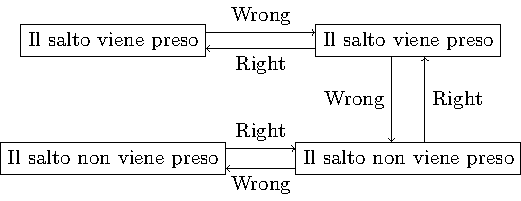
\includegraphics{dynamic_prediction}
    \caption{Esempio predizione dinamica}
    \label{fig:dynamic_prediction}
\end{figure}

Queste predizioni sono salvate in una tabella di predizione associativa, dove ad ogni indirizzo di program counter del
salto è associato il valore di relativa predizione.

\subsection{Architetture superscalari}
Quello visto sino ad ora prende il nome di pipeline lineare, non viene più utilizzato perché come visto, lo speedup
teorico è ben diverso dallo speedup reale.
Un altro problema di questa architettura è che tutte le istruzioni attraversano tutti gli stadi, il periodo di clock è
quindi determinato dallo stadio più lento (come nella multiciclo).

La soluzione è quindi introdurre non un parziale parallelismo, come nel caso della pipeline, ma un parallelismo totale,
sovrapponendo specifiche fasi delle istruzioni.
Nell'architettura che utilizzeremo come riferimento, solo la fase di execute è in parallelo:

\begin{figure}[h]
    \begin{minipage}{.5\textwidth}
        \centering
        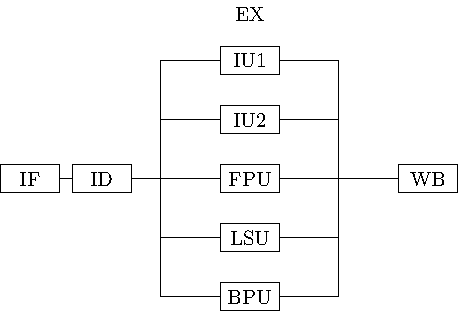
\includegraphics[width=.8\textwidth]{cpu_parallelism}
    \end{minipage}
    \begin{minipage}{.45\textwidth}
        \begin{itemize}
            \item IU1= ALU, per aritmetica intera (1 cck)
            \item IU2=ALU, per aritmetica intera, ma operazioni più complesse come moltiplicazione e divisione (2cck)
            \item FPU=ALU, per virgola mobile (4cck)
            \item BPU \textit{Branch Prediction Unit}
            \item LSU \textit{Load Store Unit}
        \end{itemize}
    \end{minipage}
    \caption{Architettura di riferimento}
\end{figure}

Ipotizziamo che allo stadio di execute venga emessa solo una istruzione alla volta (ID), una volta messe in esecuzione,
è sono eseguite in parallelo.

\subsubsection{Problemi dell'architettura}
\begin{enumerate}
    \item Date due istruzioni $i$ e $j$, se con $i$ che precede $j$, se $i$ impiega più cicli di clock di $j$ ad essere eseguita,
        l'ordine di completamento può essere invertito.
    \item Può accadere che due istruzioni nello stesso istante richiedano di passare alla fase di writeback, generando
        un conflitto di risorse.
\end{enumerate}


\end{document}
